\section{Results}\label{sec:results}

This section presents the testing results of the proposed solution.
First, hyper-parameters are tested in order to determine their reasonable values in subsection~\ref{subsec:hyper-parameters}.
Next, using these values, the results of performance tests are presented subsection~\ref{subsec:performance}.
Lastly, the best-obtained solutions are visualized in the section~\ref{subsec:visualization}.

\subsection{Hyper-parameters}\label{subsec:hyper-parameters}

\begin{table}[]
    \begin{tabular}{|l|l|}
        \hline
        & optimal value                         \\ \hline
        population size         & $50$ or $100$ times the instance size \\ \hline
        overlapping penalization constant & \begin{tabular}[c]{@{}l@{}}between $2$ and $5$ times\\ the layout diagonal length\end{tabular} \\ \hline
        maximum wild card count & 1                                     \\ \hline
    \end{tabular}
    \caption{Hyperparameters and their optimal values.}
    \label{tab:hyperparameters-opt}
\end{table}

\subsubsection*{Population size}

Population size is tested in order to determine a reasonable value called \textit{population scaling factor}.
This value determines the size of the population with respect to the instance size.
Thus, for instance, with size $N$ and scaling factor $k$, population size is determined as
$kN$.
This means that the population size is linear with respect to the instance size.

Results for two random instances can be seen in figure~\ref{fig:pop-size}.
From it, we can deduce that scaling factor $10$ does not allow
the population objective average to decrease to the levels comparable to scaling factors $50$ and $100$.
This might imply that the scaling factor $10$ is insufficient to represent knowledge gathered over time
in the genetic approach.
Also, researches in~\cite{goncalvesBiasedRandomkeyGenetic2015} solving UA-FLP using BRKGA
similarly obtained their best results for scaling factor $100$.

The conclusion is that using scaling factor between $50$ and $100$ is sufficient, with bias towards $100$
for obtaining better average objective performance.
However, increasing the scaling factor leads to slower computation speed as every population contains
more individuals for which genetic operators and reproductive plan must be computed.

\subsubsection*{Overlapping penalization constant}

It is not desirable to produce a solution where paintings overlap.
Thus, \textit{overlapping penalization constant} is used to penalize
individuals that represent such a solution.
How this constant is used inside the objective function is in equation~\ref{eq:objective}.

The optimal value where the penalization is strong enough
to uproot overlapping solutions from the population and, at the same time, low enough
to be at the same scale as other parts of the objective value are tested on two instances – random\_10 and packing\_10.

Value tested for \textit{overlapping penalization constant} is proportional to the diagonal length of the layout to which paintings are placed.
This way, it contains the information about layout dimensions.
Thus, if $w$ is width and $h$ is height of the layout, tested value is called $k$ which determines
\textit{overlapping penalization constant} as $k\sqrt{w^2 + h^2}$.

Results are in figure~\ref{fig:overlapping-penalization} for two instances.
From it, we can deduce that the optimal value for \textit{overlapping penalization constant} is between $2$ and $5$ times the length of the layout diagonal.

\subsubsection*{Maximum wild card count}
Maximum wild card count determines the maximum number of wild card symbol $*$ that a decoded individual can contain.
It is recommended to keep this parameter very low or even set it to zero.
Reason is that if the parameter is high, computation time might increase if $*$ will spread in population.
For instance os size $N$, if the wild card count in unconstrained, i.e., it is set to maximum possible number $N-1$,
then one individual decodes to $2^{N-1}$ values.

Results for computation time are in figure~\ref{fig:computation-time}.
From it, we can see


\afterpage{%
    \clearpage% Flush earlier floats (otherwise order might not be correct)
    \begin{landscape}% Landscape page
        \begin{figure}
            \centering
            \subfloat{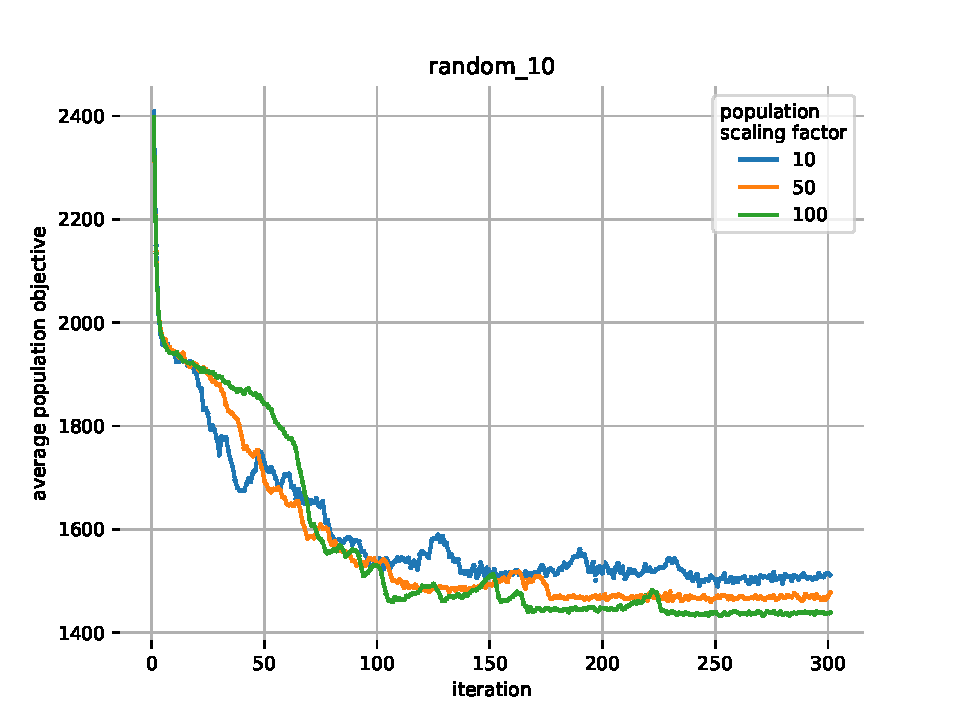
\includegraphics[width=0.8\textwidth]{pop_size_random_10}\label{subfig:pop-size-random-10}}
            \subfloat{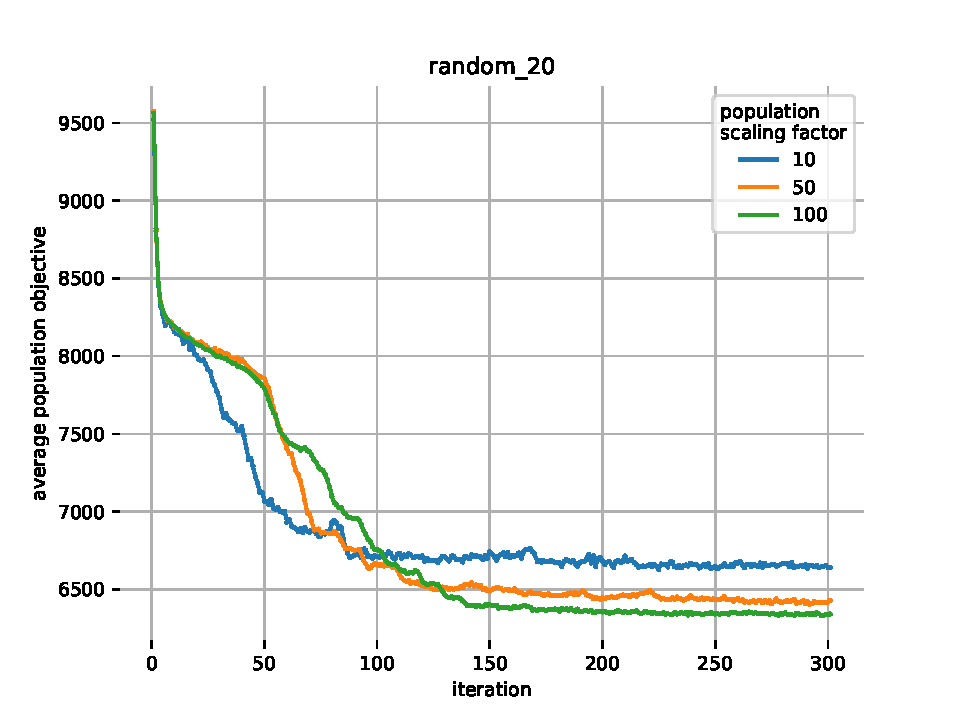
\includegraphics[width=0.8\textwidth]{pop_size_random_20}\label{subfig:pop-size-random-20}}
            \caption[Testing population scaling factor]{Testing population scaling factor at two random instances.
            For population scaling factor $k$ and instance of size $N$, i.e. the number of paintings, population size is $kN$.}
            \label{fig:pop-size}%
        \end{figure}
    \end{landscape}
    \clearpage% Flush page
}

\afterpage{%
    \clearpage% Flush earlier floats (otherwise order might not be correct)
    \begin{landscape}% Landscape page
        \begin{figure}
            \centering
            \subfloat{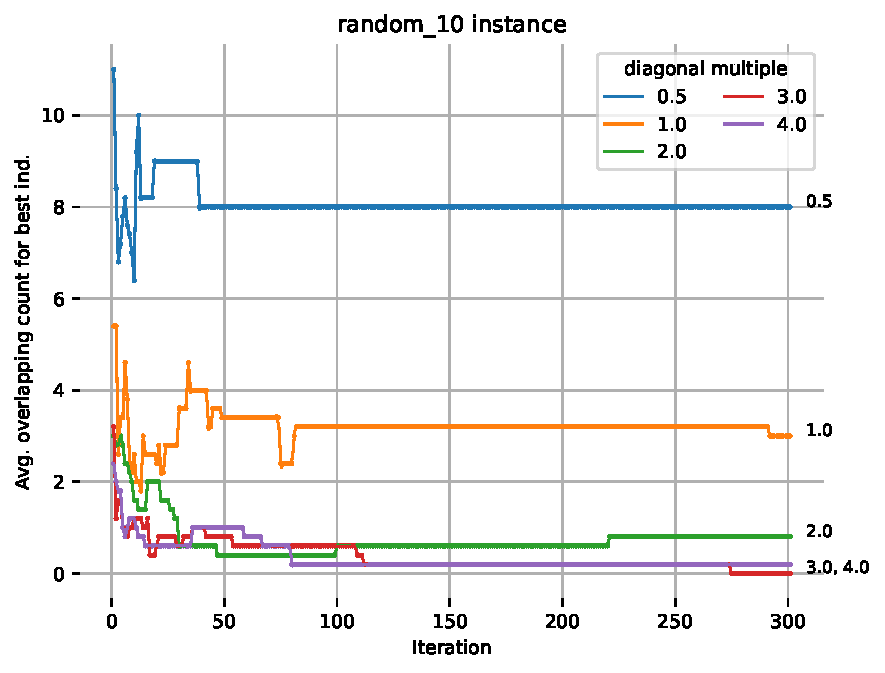
\includegraphics[width=0.8\textwidth]{overlapping_penalization_constant_random_10}\label{subfig:overlapping-random-10}}
            \subfloat{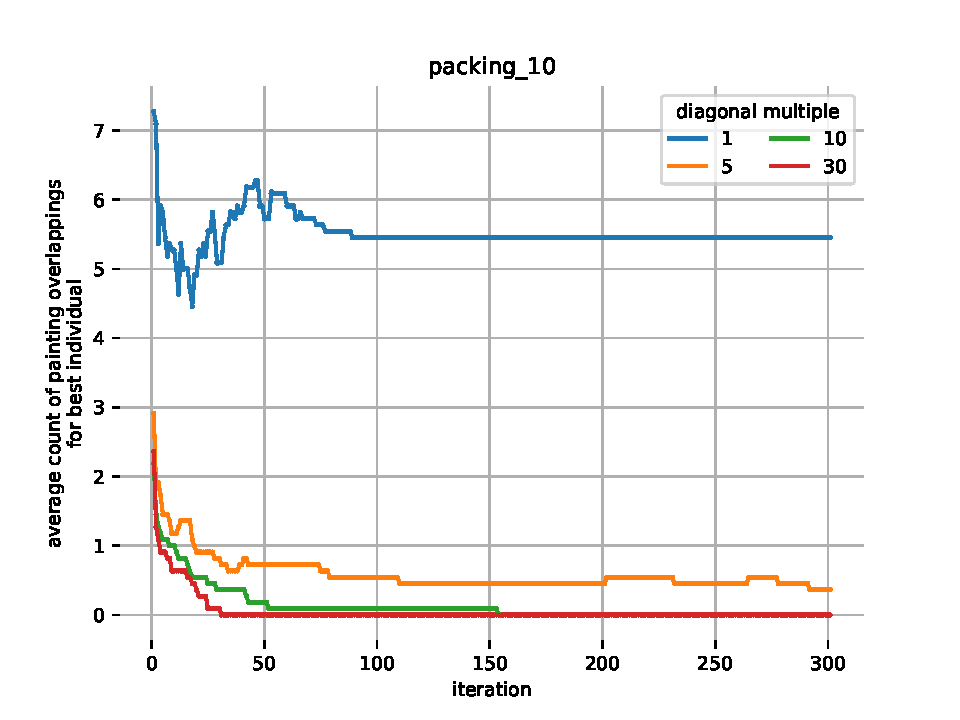
\includegraphics[width=0.8\textwidth]{overlapping_penalization_constant_packing_10}\label{subfig:overlapping-packing-10}}
            \caption[Testing population overlapping penalization constant]{Testing overlapping penalization contanst.
            Diagonal multiple $k$ determines overlapping penalization constant as $k\sqrt{w^2 + h^2}$, where $w$, $h$ are dimension of the layout.}
            \label{fig:overlapping-penalization}%
        \end{figure}
    \end{landscape}
    \clearpage% Flush page
}

\afterpage{%
    \clearpage% Flush earlier floats (otherwise order might not be correct)
    \begin{landscape}% Landscape page
        \begin{figure}
            \centering
            \subfloat{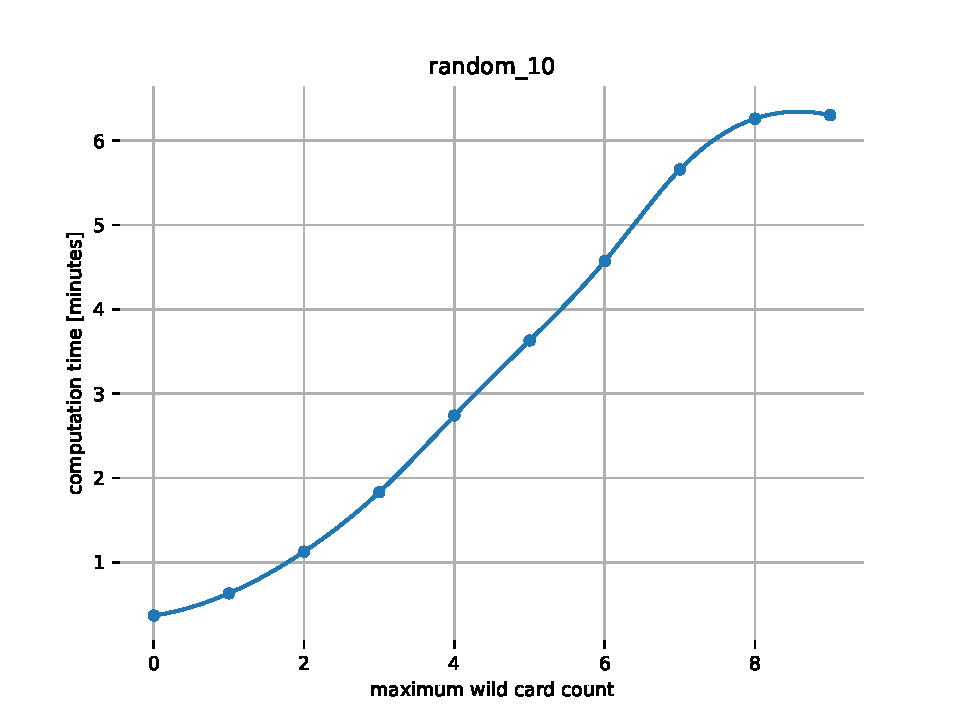
\includegraphics[width=0.8\textwidth]{computation_time_random_10}\label{subfig:computation-time-10}}
%            \subfloat{\includegraphics[width=0.8\textwidth]{computation_time_random_20}\label{subfig:computation-time-20}}
            \caption[Testing computation speed]{Testing computation speed for increasing maximum wild card count.}
            \label{fig:computation-time}%
        \end{figure}
    \end{landscape}
    \clearpage% Flush page
}

\subsection{Performance}\label{subsec:performance}

\afterpage{%
    \clearpage% Flush earlier floats (otherwise order might not be correct)
    \begin{landscape}% Landscape page
        \begin{figure}
            \centering
            \subfloat{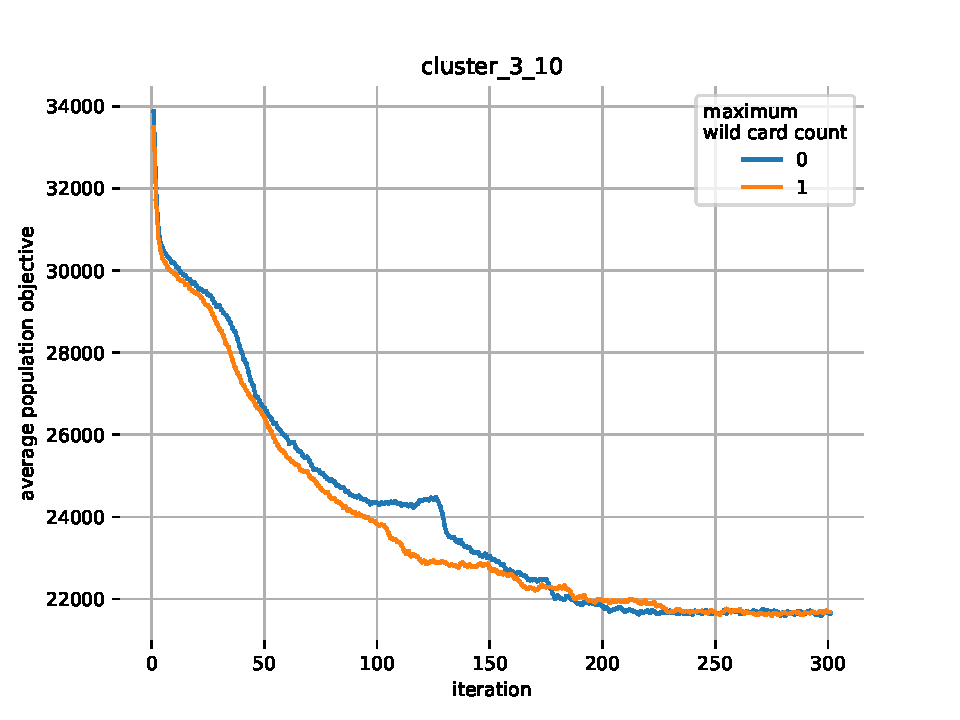
\includegraphics[width=0.8\textwidth]{cluster_3_10}\label{subfig:cluster-3-10}}
            \subfloat{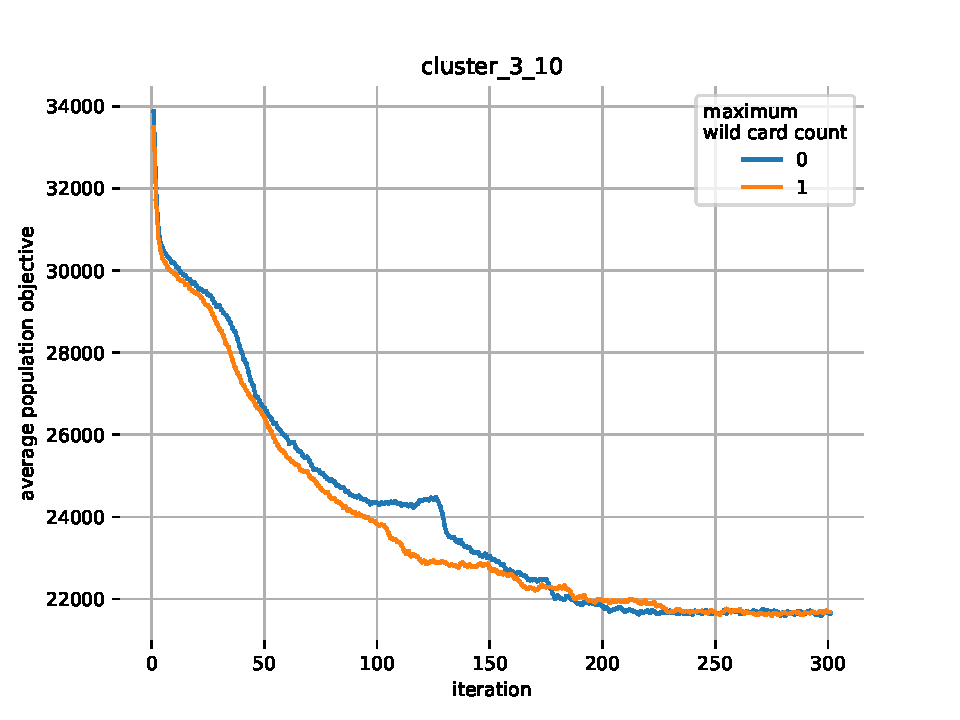
\includegraphics[width=0.8\textwidth]{cluster_3_10}\label{subfig:cluster-3-10}}
            \caption[Testing clustering dataset]{Testing clustering dataset performance with a different maximum wildcard count.}
            \label{fig:cluster}%
        \end{figure}
    \end{landscape}
    \clearpage% Flush page
}

\subsection{Visualization}\label{subsec:visualization}

\afterpage{%
    \clearpage% Flush earlier floats (otherwise order might not be correct)
    \begin{landscape}% Landscape page
        \begin{figure}
            \centering
            \subfloat[brute-force]{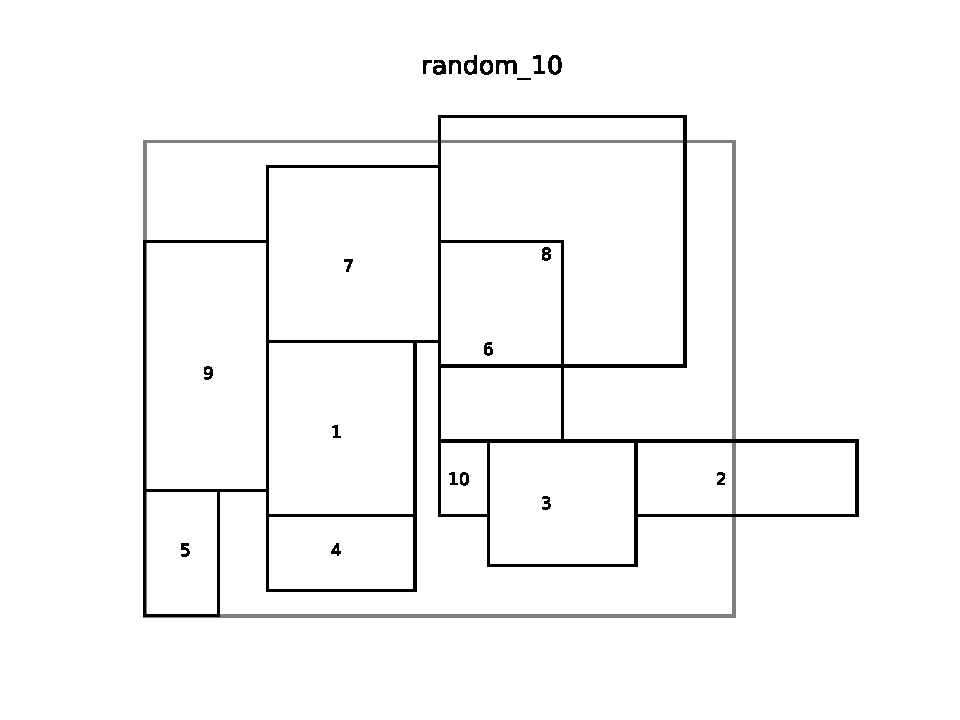
\includegraphics[width=0.9\textwidth]{visualization_random10_brute}\label{subfig:random10-brute}}
            \subfloat[proposed solution]{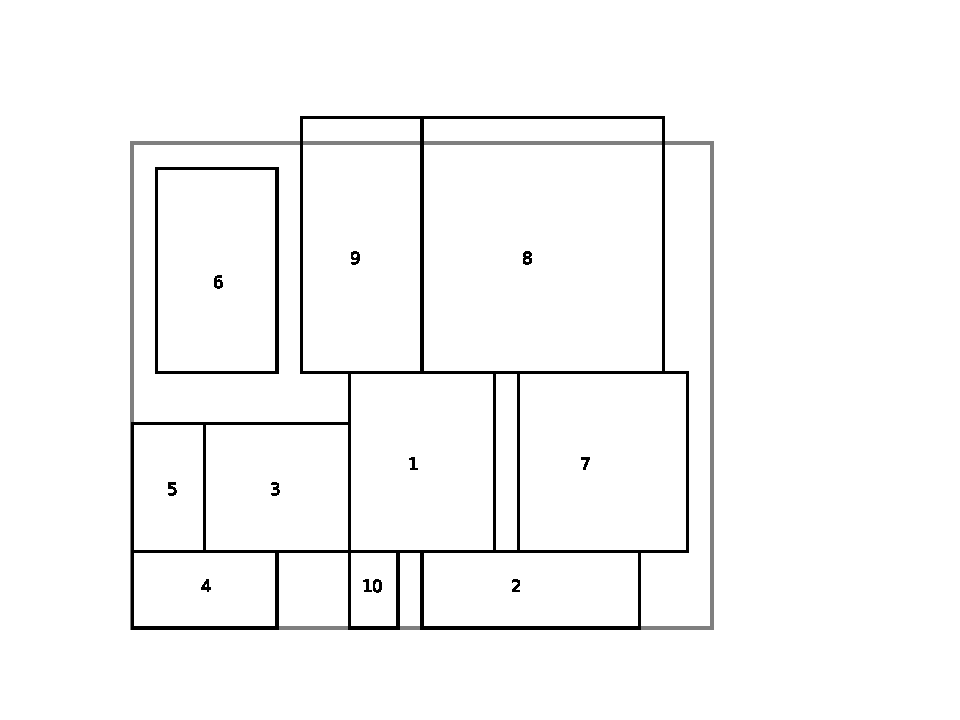
\includegraphics[width=0.9\textwidth]{visualization_random10_ga}\label{subfig:random10-ga}}
            \caption[Instance random\_10 visualization]{Visualization of best result of proposed solution and brute-force for random\_10 instance.}
            \label{fig:visualization-random10}%
        \end{figure}
    \end{landscape}
    \clearpage% Flush page
}

\afterpage{%
    \clearpage% Flush earlier floats (otherwise order might not be correct)
    \begin{landscape}% Landscape page
        \begin{figure}
            \centering
            \subfloat[brute-force]{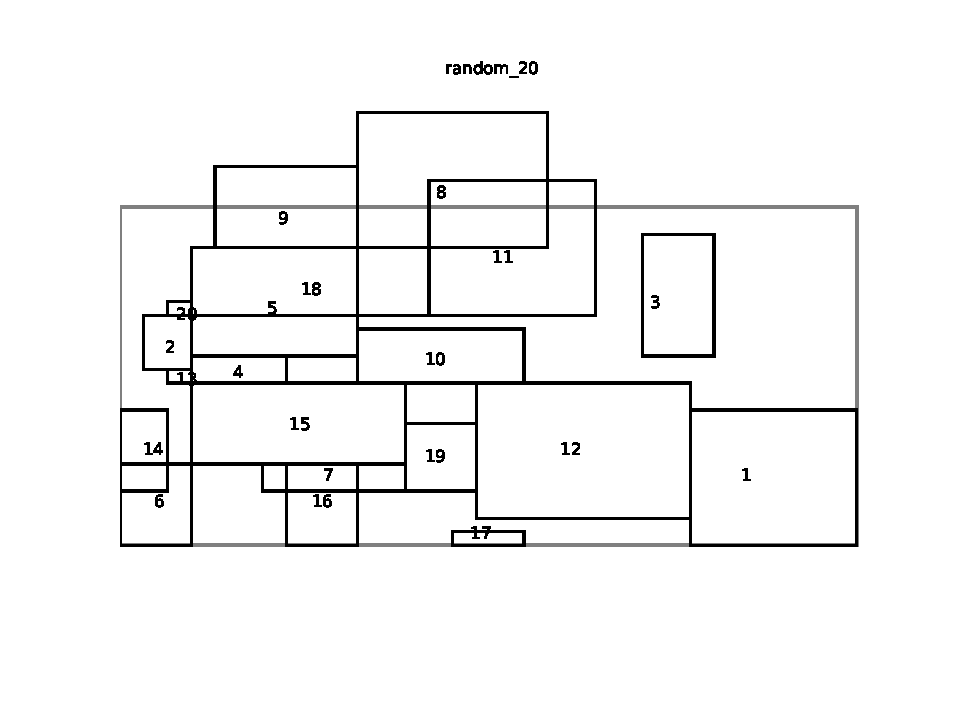
\includegraphics[width=0.8\textwidth]{visualization_random20_brute}\label{subfig:random20-brute}}
            \subfloat[proposed solution]{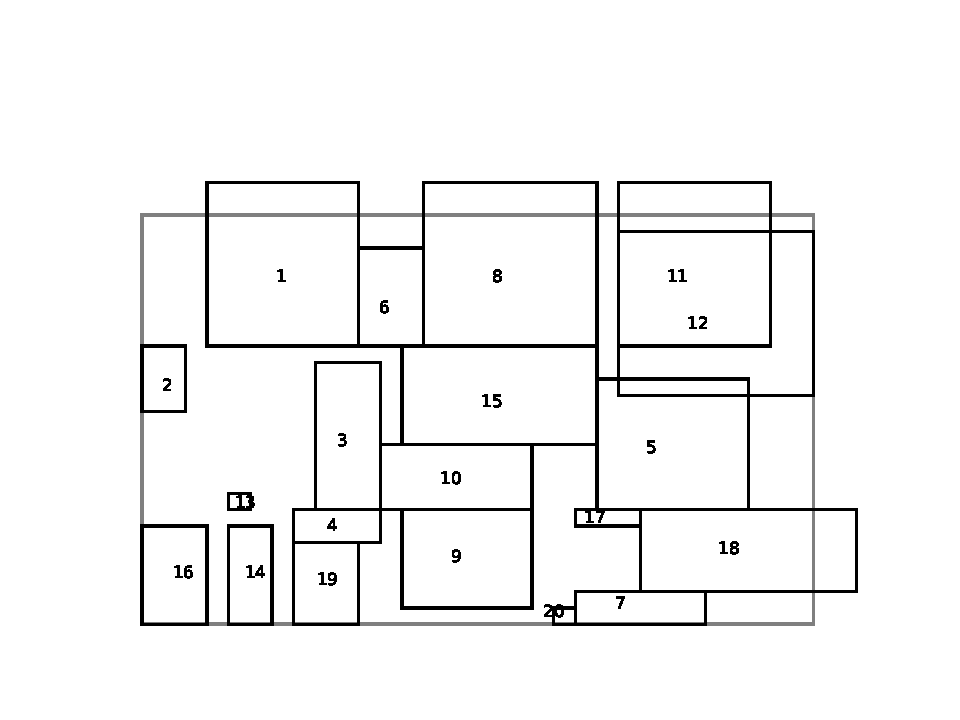
\includegraphics[width=0.8\textwidth]{visualization_random20_ga}\label{subfig:random20-ga}}
            \caption[Instance random\_20 visualization]{Visualization of best result of proposed solution and brute-force for random\_20 instance.}
            \label{fig:visualization-random20}%
        \end{figure}
    \end{landscape}
    \clearpage% Flush page
}

\afterpage{%
    \clearpage% Flush earlier floats (otherwise order might not be correct)
    \begin{landscape}% Landscape page
        \begin{figure}
            \centering
            \subfloat{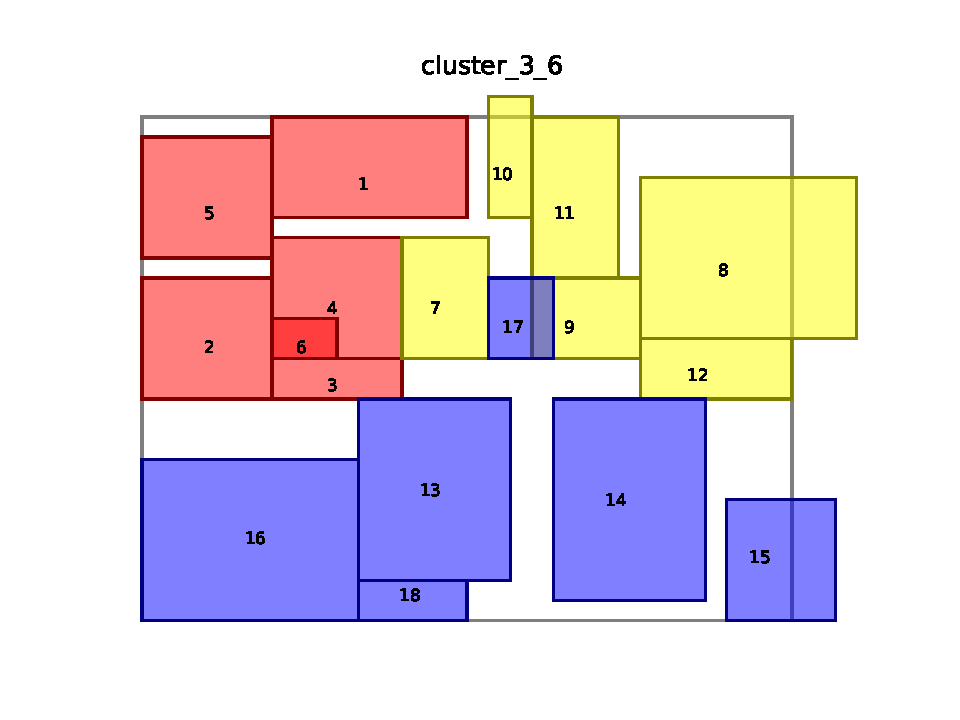
\includegraphics[width=0.8\textwidth]{visualization_cluster_3_6_ga}\label{subfig:cluster-3-6-ga}}
            \subfloat{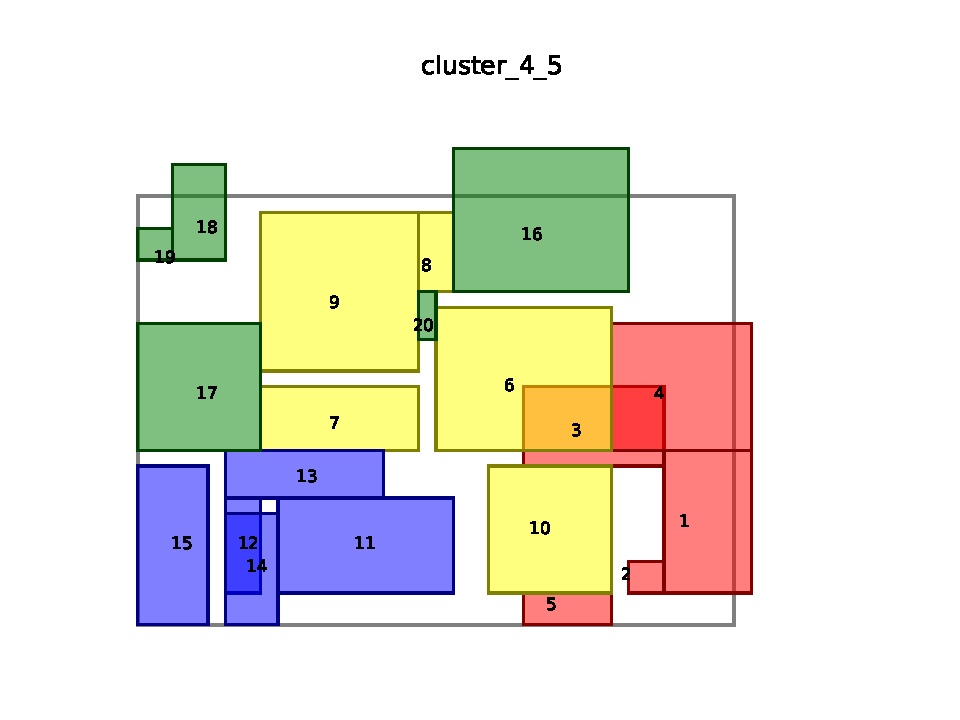
\includegraphics[width=0.8\textwidth]{visualization_cluster_4_5_ga}\label{subfig:cluster-4-5-ga}}
            \caption[Clustering instances visualization]{Visualization of the best result of proposed solution for instances cluster\_3\_6 and cluster\_4\_5.}
            \label{fig:visualization-cluster}%
        \end{figure}
    \end{landscape}
    \clearpage% Flush page
}

\afterpage{%
    \clearpage% Flush earlier floats (otherwise order might not be correct)
    \begin{landscape}% Landscape page
        \begin{figure}
            \centering
            \subfloat{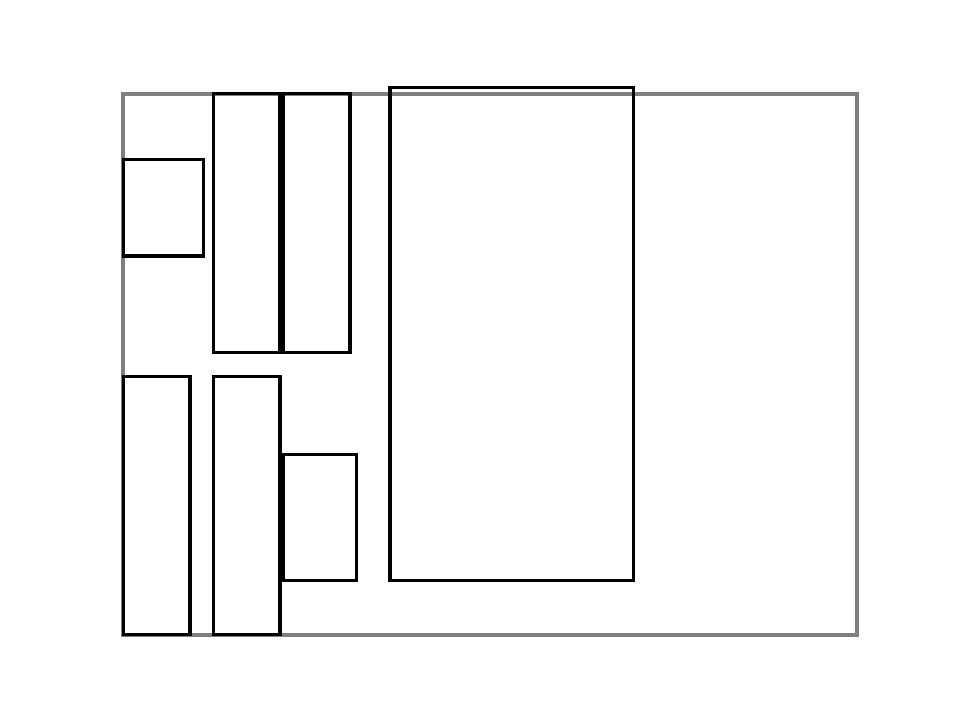
\includegraphics[width=0.8\textwidth]{visualization_london_nationa_gallery_ga}\label{subfig:london-gallery-ga}}
            \caption[London National Gallery visualization]{Visualization of the London National Gallery wall dataset.}
            \label{fig:visualization-cluster}%
        \end{figure}
    \end{landscape}
    \clearpage% Flush page
}
